\documentclass[11pt]{article}
\usepackage{ovariansubtypes}
\usepackage[figurename=Supplementary Figure]{caption}
\title{ \textbf{Genomic landscapes of endometrioid and mucinous ovarian cancers and morphologically similar tumor types}}
\date{}
% change footnote to dagger
\makeatletter
\def\@fnsymbol#1{\ensuremath{\ifcase#1\or \dagger\or \ddagger\or
      \mathsection\or \mathparagraph\or \|\or **\or \dagger\dagger
    \or \ddagger\ddagger \else\@ctrerr\fi}}
\makeatother
% same footnote for second corresponding author
\newcommand*\colast[1][\value{footnote}]{\footnotemark[#1]}
\newcommand*\cofirst[1][\value{footnote}]{\footnotemark[#1]}
\author[1]{Dorothy Hallberg\thanks{These authors contributed equally.}}
\author[1]{Alice C. Eastman\cofirst}
\author[1]{Shashikant Koul\cofirst}
\author[1]{Daniel C. Bruhm}
\author[1]{Eniko Papp}
\author[2]{Simon Davenport}
\author[1]{Vilmos Adleff}
\author[1]{Leonardo Ferreira}
\author[1]{Noushin Niknafs}
\author[1]{Jamie E. Medina}
\author[1]{Stephen Cristiano}
\author[1]{Carolyn Hruban}
\author[1]{Jacob Fiksel}
\author[1]{Kaui P. Lebarbenchon}
\author[1]{Luis Aparicio}
\author[1]{Nicholas A. Vulpescu}
\author[3]{Kuan-Ting Kuo}
\author[1,4]{Nita Ahuja}
\author[5]{Ronny Drapkin}
\author[5]{Euihye Jung}
\author[5]{Sarah Kim}
\author[6]{Mark A. Eckert}
\author[6]{Ernst Lengyel}
\author[7]{Kentaro Nakayama}
\author[1,8]{Ayse Ayhan}
\author[1]{Ie-Ming Shih}
\author[2]{Tian-Li Wang}
\author[9]{Ofer Lavie}
\author[10]{Gad Rennert}
\author[1]{Hariharan Easwaran}
\author[1]{Stephen R. Baylin}
\author[2]{Michael F. Press}
\author[1]{Victor E. Velculescu\thanks{To whom correspondence should be addressed:\ velculescu@jhmi.edu (V.E.V.) and rscharpf@jhu.edu (R.B.S.).}}
\author[1, 11]{Robert B. Scharpf\colast}

\affil[1]{The Sidney Kimmel Comprehensive Cancer Center, Johns Hopkins University School of Medicine, Baltimore, MD, USA\vspace{0.5em}}
\affil[2]{Department of Pathology, Norris Comprehensive Cancer Center, University of Southern California, Los Angeles, CA, USA\vspace{0.5em}}
\affil[3]{Department of Pathology, National Taiwan University Hospital, Taipei, Taiwan\vspace{0.5em}}
\affil[4]{Department of Pathology and Surgery, Yale University School of Medicine, New Haven, CT, USA\vspace{0.5em}}
\affil[5]{Penn Ovarian Cancer Research Center and Department of Obstetrics and Gynecology,  Division of Gynecologic Oncology,  Hospital of the University of Pennsylvania and Perelman School of Medicine, University of Pennsylvania, Philadelphia, PA, USA\vspace{0.5em}}
\affil[6]{Department of Obstetrics and Gynecology and Section of Gynecologic Oncology,  The University of Chicago, Chicago, IL, USA\vspace{0.5em}}
\affil[7]{Department of Gynecology and Obstetrics, Shimane University, Izumo, Japan\vspace{0.5em}}
\affil[8]{Department of Pathology, Seirei Mikatahara Hospital, Hamamatsu, Japan;  Department of Tumor Pathology, Hamamatsu University School of Medicine, Hamamatsu, Japan; Department of Molecular Pathology, Hiroshima University School of Medicine, Hiroshima, Japan\vspace{0.5em}}
\affil[9]{Division of Obstetrics and Gynecology, Carmel Medical Center, Haifa, Israel\vspace{0.5em}}
\affil[10]{Department of Community Medicine and Epidemiology,  Carmel Medical Center and B. Rappaport Faculty of Medicine, Technion-Israel Institute of Technology, Haifa, Israel\vspace{0.5em}}
\affil[11]{Department of Biostatistics,  Johns Hopkins Bloomberg School of Public Health, Baltimore, MD, USA}

\raggedbottom

%%% Local Variables:
%%% mode: LaTeX
%%% TeX-master: t
%%% End:

\usepackage[sf,bf,medium,compact]{titlesec}
\usepackage{pifont}

\begin{document}
\thispagestyle{empty}

\maketitle

\clearpage

\begin{figure}
\includegraphics[width=\textwidth]{../docs/figure/ext-figure1.Rmd/ext\_fig1comb-1.pdf}
\caption{\textbf{Relationship between tumor purity and number of somatic mutations.}  (\textbf{a}) Tumor purity for multiple histological tumor types were estimated using FACETS. Samples that FACETS did not process due to undetectable copy number changes are marked with an `{\footnotesize\ding{53}}'.
  (\textbf{b}) Patients with uterine endometrioid adenocarcinomas were more than twice as likely to have a hypermutator defect compared to patients with other cancers, including patients with ovarian endometrioid cancer (95\% CI: 1.1 - 4.2-fold increase).}
\label{fig:sfig1}
\end{figure}

\begin{figure}
  \includegraphics[width=\textwidth]{../docs/figure/ext-figure2.Rmd/ext\_fig2-1.pdf}
  %\vspace{-9em}
\caption{\textbf{Mutations in ESR1 at Tyr537 and Leu536.} \textit{ESR1} mutations identified in two patients with uterine endometrioid carcinomas occurred at Tyr537, a hotspot most commonly associated with aromatase inhibitor resistance in patients with breast cancer patients, and Leu536.
This hotspot is located in close proximity to the region of the estrogen receptor that is important for ligand-dependent transcriptional function.
The Tyr537 mutations cause a conformational change that constitutively activates the receptor independent of estrogen receptor binding.
The Tyr537 residue is highlighted in blue in a three dimensional view of the ESR1 protein (bottom).
Due to its physical proximity to the Tyr537 hotspot, the Leu536 mutation is likely to have the same activating effect on the estrogen receptor.}
\label{fig:sfig2}
\end{figure}

\begin{figure}
\includegraphics[width=\textwidth]{../docs/figure/ext-figure3.Rmd/ext\_fig3-1.pdf}
\caption{\textbf{Mutation signature analyses.}
  \textbf{(a)} Mutation signatures for ovarian and uterine endometrioid carcinomas visualized with unsupervised clustering.
  \textbf{(b)} Mutation signatures for ovarian and GI mucinous carcinomas.
  The intensity of the heatmap colors indicates the percentage of the overall mutational profile for a sample that is explained by the mutation signature.}
\label{fig:sfig3}
\end{figure}

\begin{figure}
\includegraphics[width=\textwidth]{../docs/figure/ext-figure4-7.Rmd/ovarian\_endometrioid-1.pdf}
\caption{\textbf{Circos plots of ovarian endometrioid carcinoma samples.}
Circos plots depict copy number alterations (black line segments interior of the chromosomes) as well as intra- and inter-chromosomal rearrangements (blue lines that connect different portions of the cancer genome).}
\label{fig:sfig4}
\end{figure}

\begin{figure}
  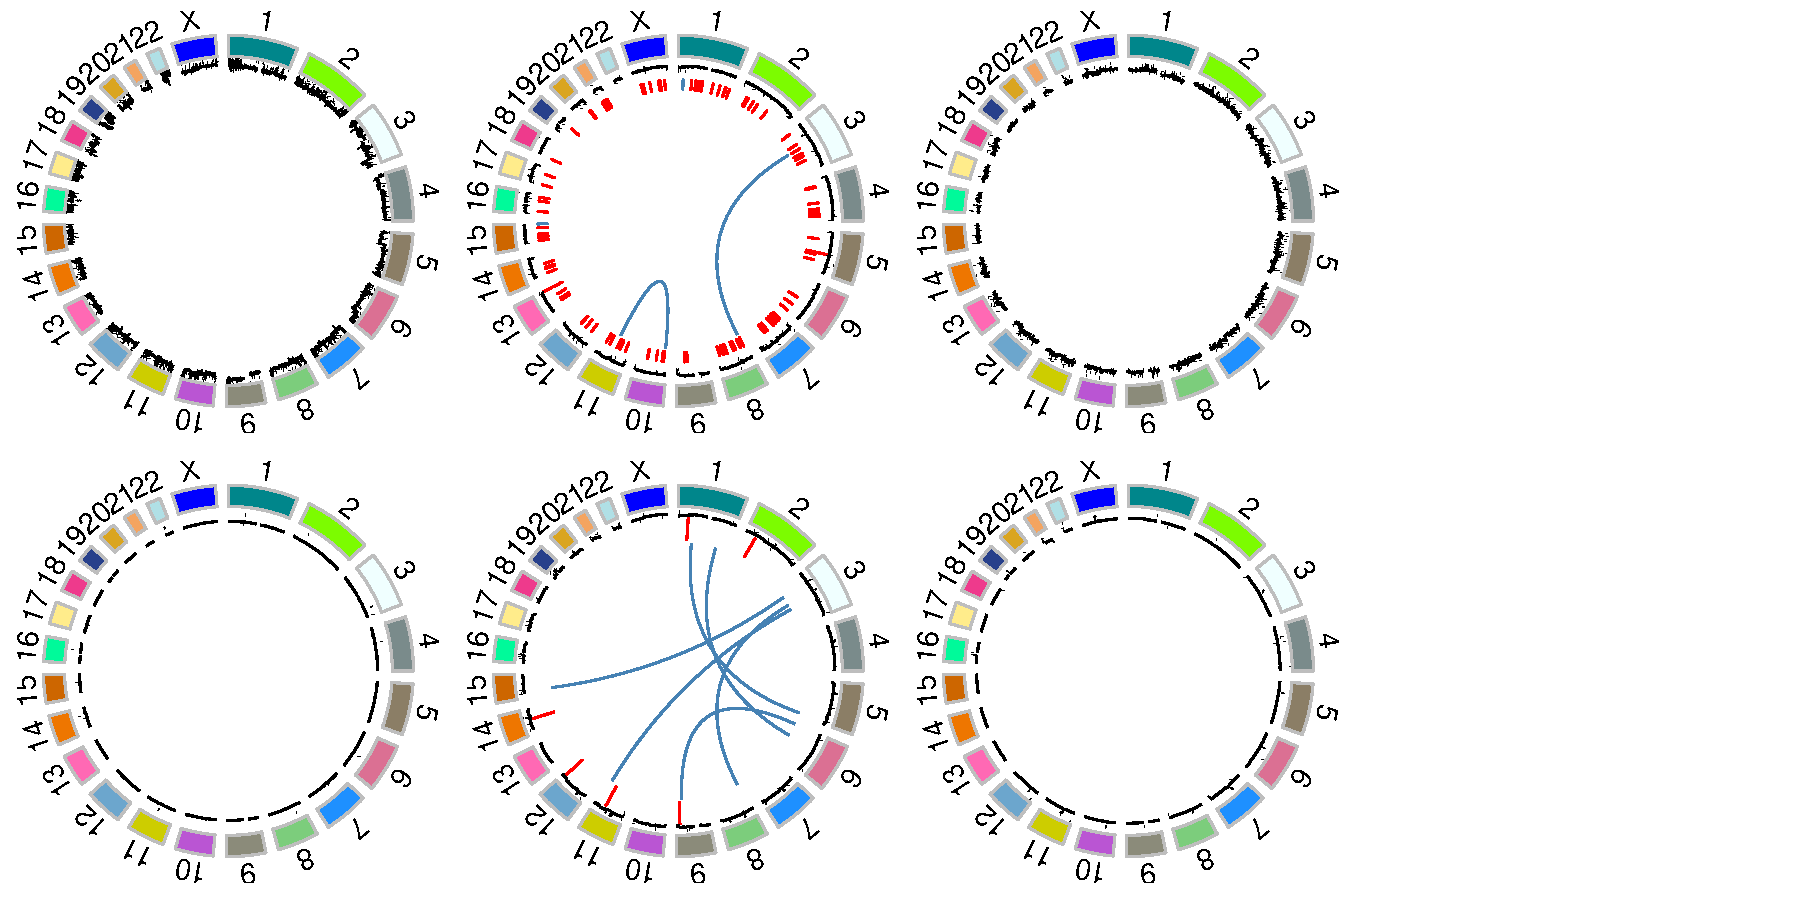
\includegraphics[width=\textwidth]{../docs/figure/ext-figure4-7.Rmd/uterine-1.pdf}
  \caption{\textbf{Circos plots of uterine endometrioid carcinoma samples.}}
  \label{fig:sfig5}
\end{figure}

\begin{figure}
\includegraphics[width=\textwidth]{../docs/figure/ext-figure4-7.Rmd/ovarian\_mucinous-1.pdf}
\caption{\textbf{Circos plots of ovarian mucinous carcinoma samples.}}
\label{fig:sfig6}
\end{figure}


\begin{figure}
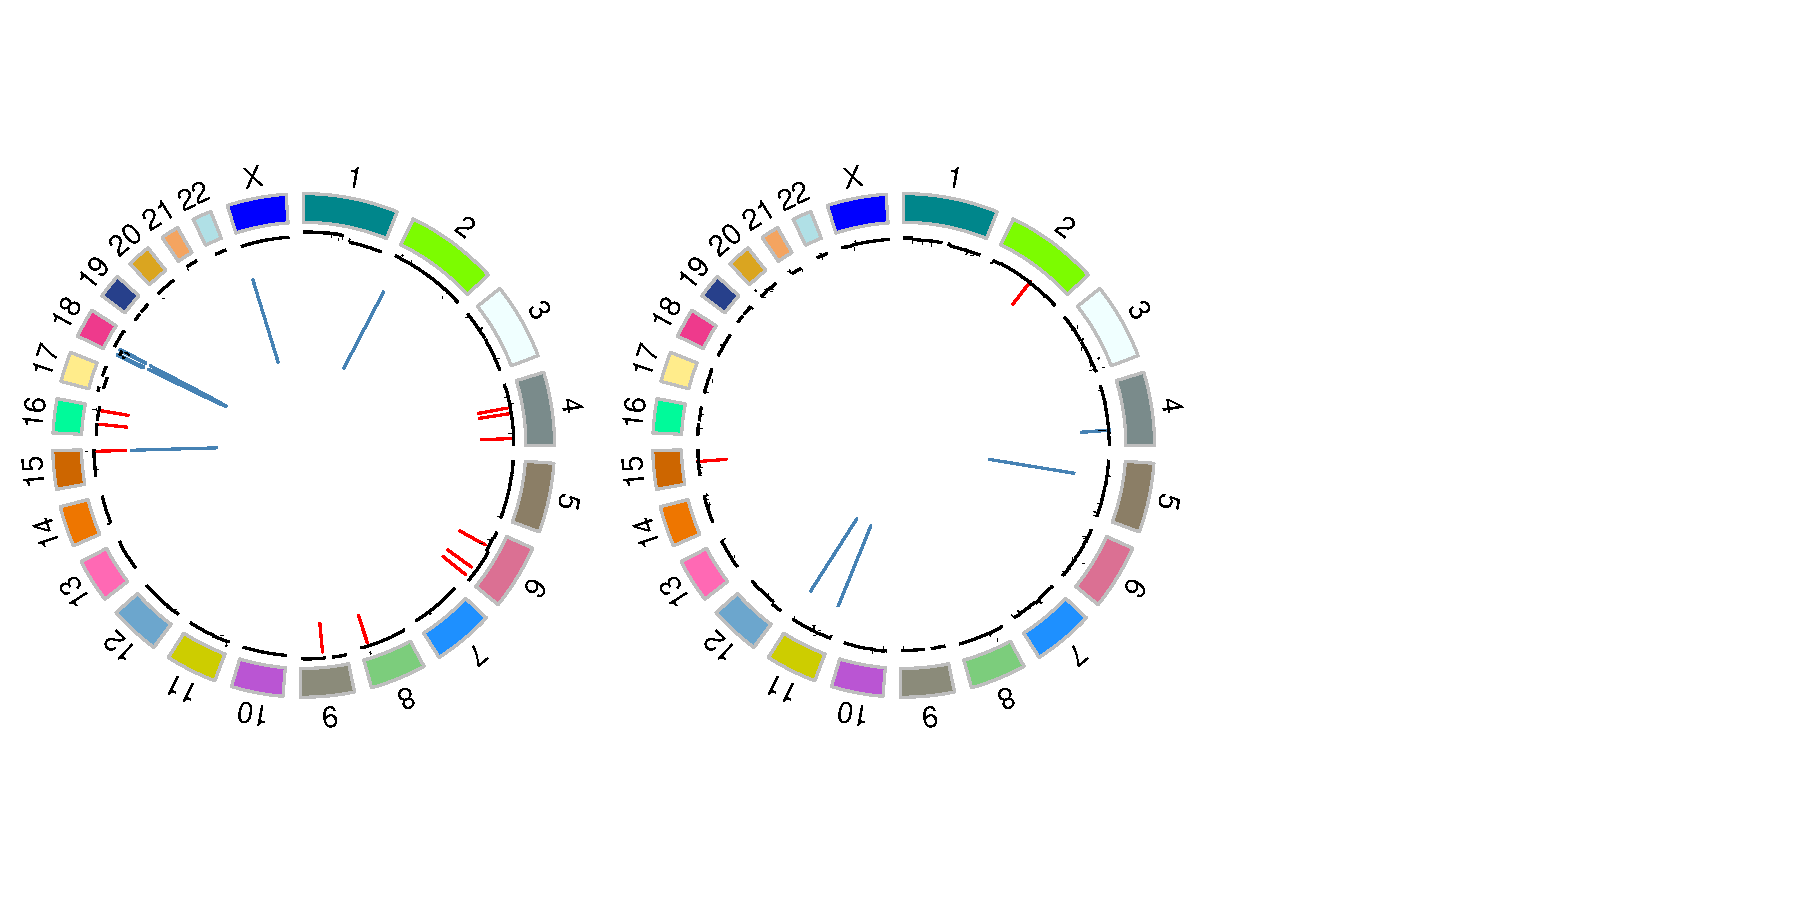
\includegraphics[width=\textwidth]{../docs/figure/ext-figure4-7.Rmd/colorectal-1.pdf}
\caption{\textbf{Circos plots of colorectal mucinous carcinoma samples}}
\label{fig:sfig7}
\end{figure}


\begin{figure}
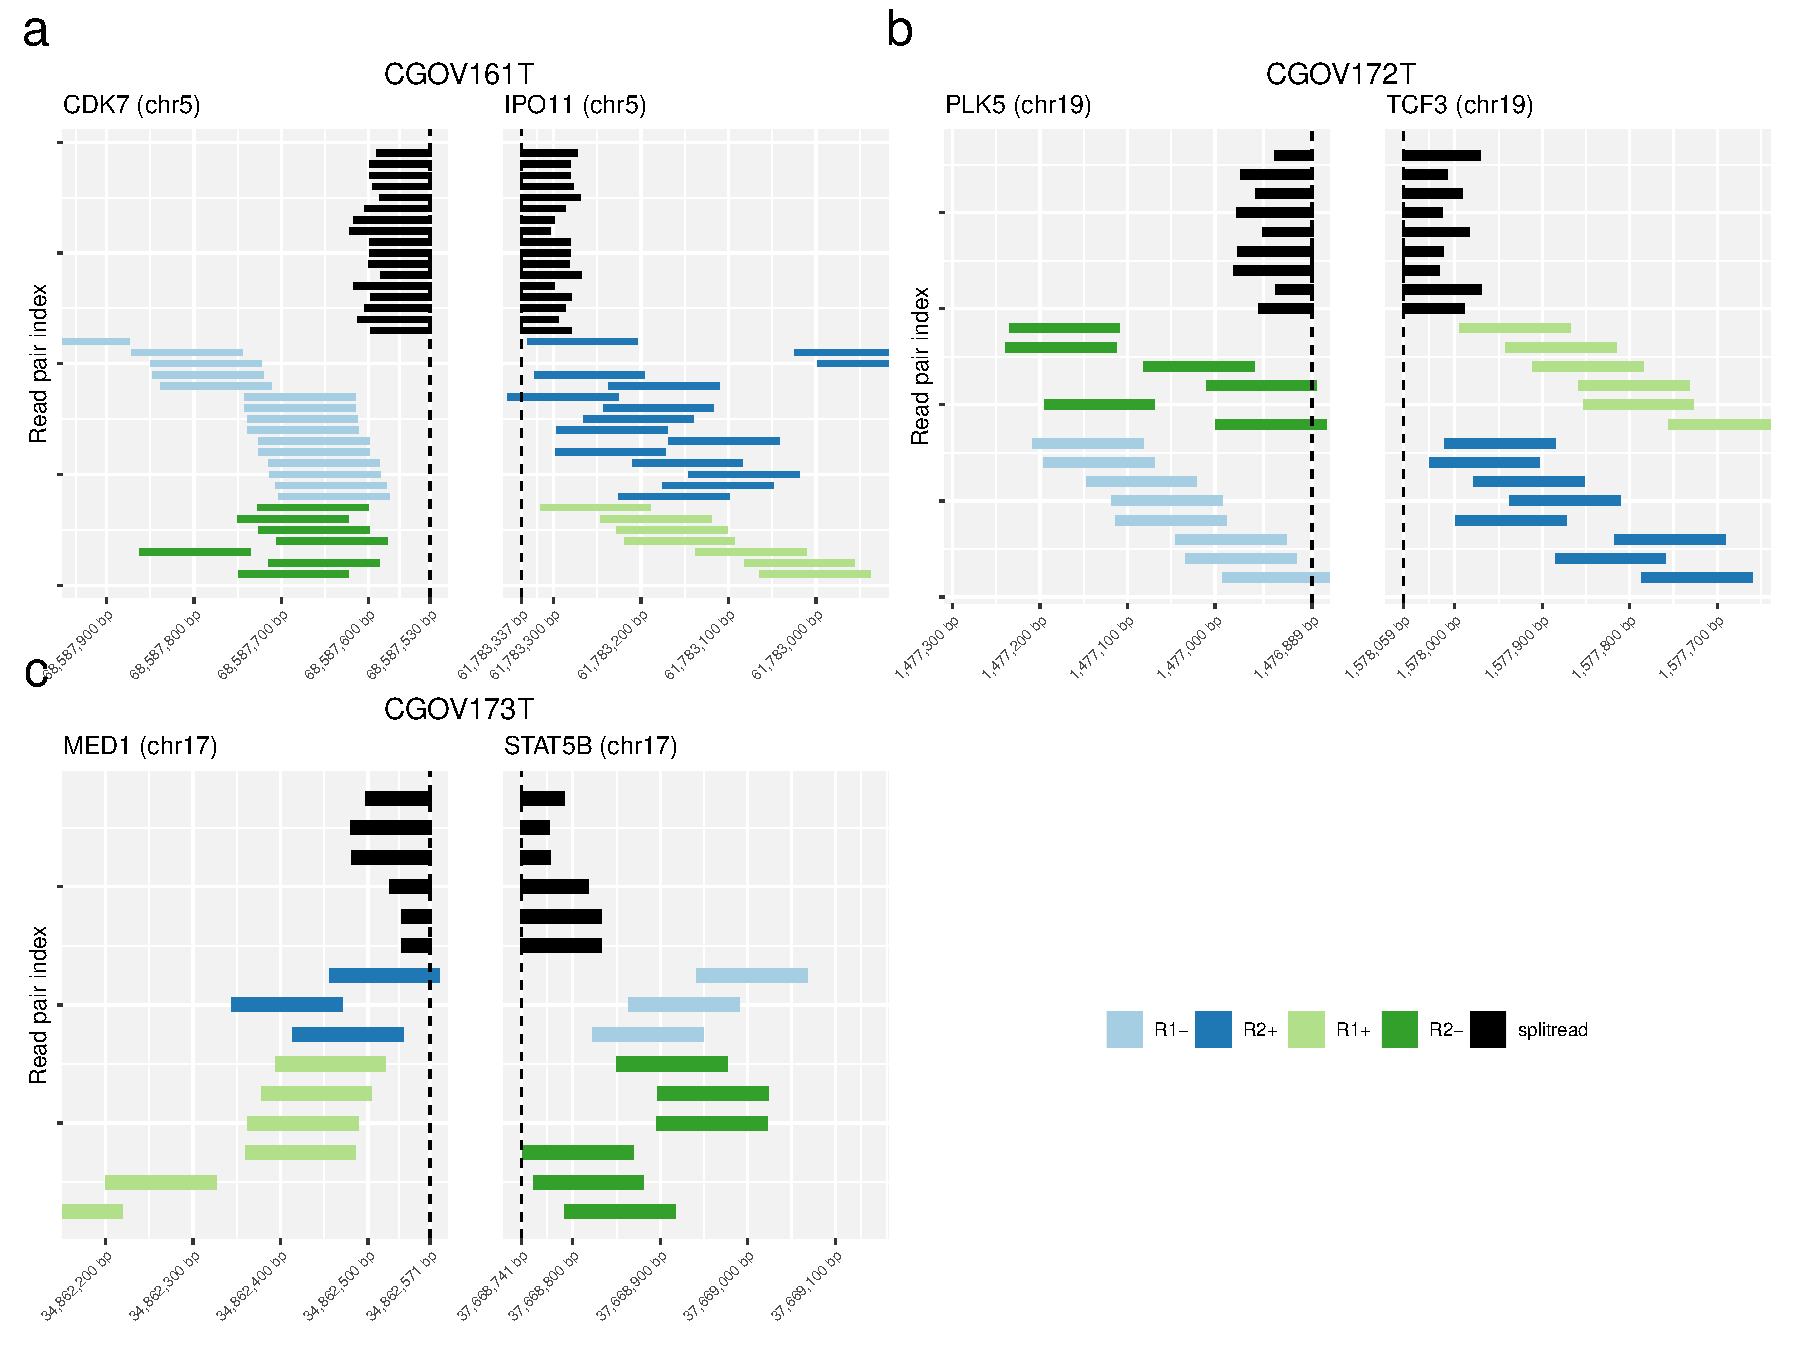
\includegraphics[width=\textwidth]{../docs/figure/ext-figure8.Rmd/ext-fig8-1.pdf}
\caption{\textbf{Rearrangements of ovarian endometrioid and ovarian mucinous carcinomas identified by \textsc{Trellis}.}
Rearrangements present in ovarian endometrioid carcinomas CGOV161T and CGOV172T (\textbf{a,b}) and an ovarian mucinous tumor CGOV173T (\textbf{c}).
Split reads that span the fusion junction are shown in black, while read pairs that reside on either side of the junction are shown in green and blue.}
\label{fig:sfig8}
\end{figure}

\begin{figure}
\includegraphics[width=\textwidth]{../docs/figure/ext-figure9.Rmd/ext\_fig9-1.pdf}
\caption{\textbf{Proportion of methylated CpG sites in ovarian and mucinous carcinomas.}
The proportion of methylated CpG sites (mean $\beta$ values $>$ 0.3) are shown for patients with mucinous stomach, mucinous pancreatic, and ovarian mucinous and ovarian endometrioid carcinomas.
Methylation was only available for one individual with colorectal mucinous carcinoma (not shown).  }
\label{fig:sfig9}
\end{figure}

\begin{figure}
  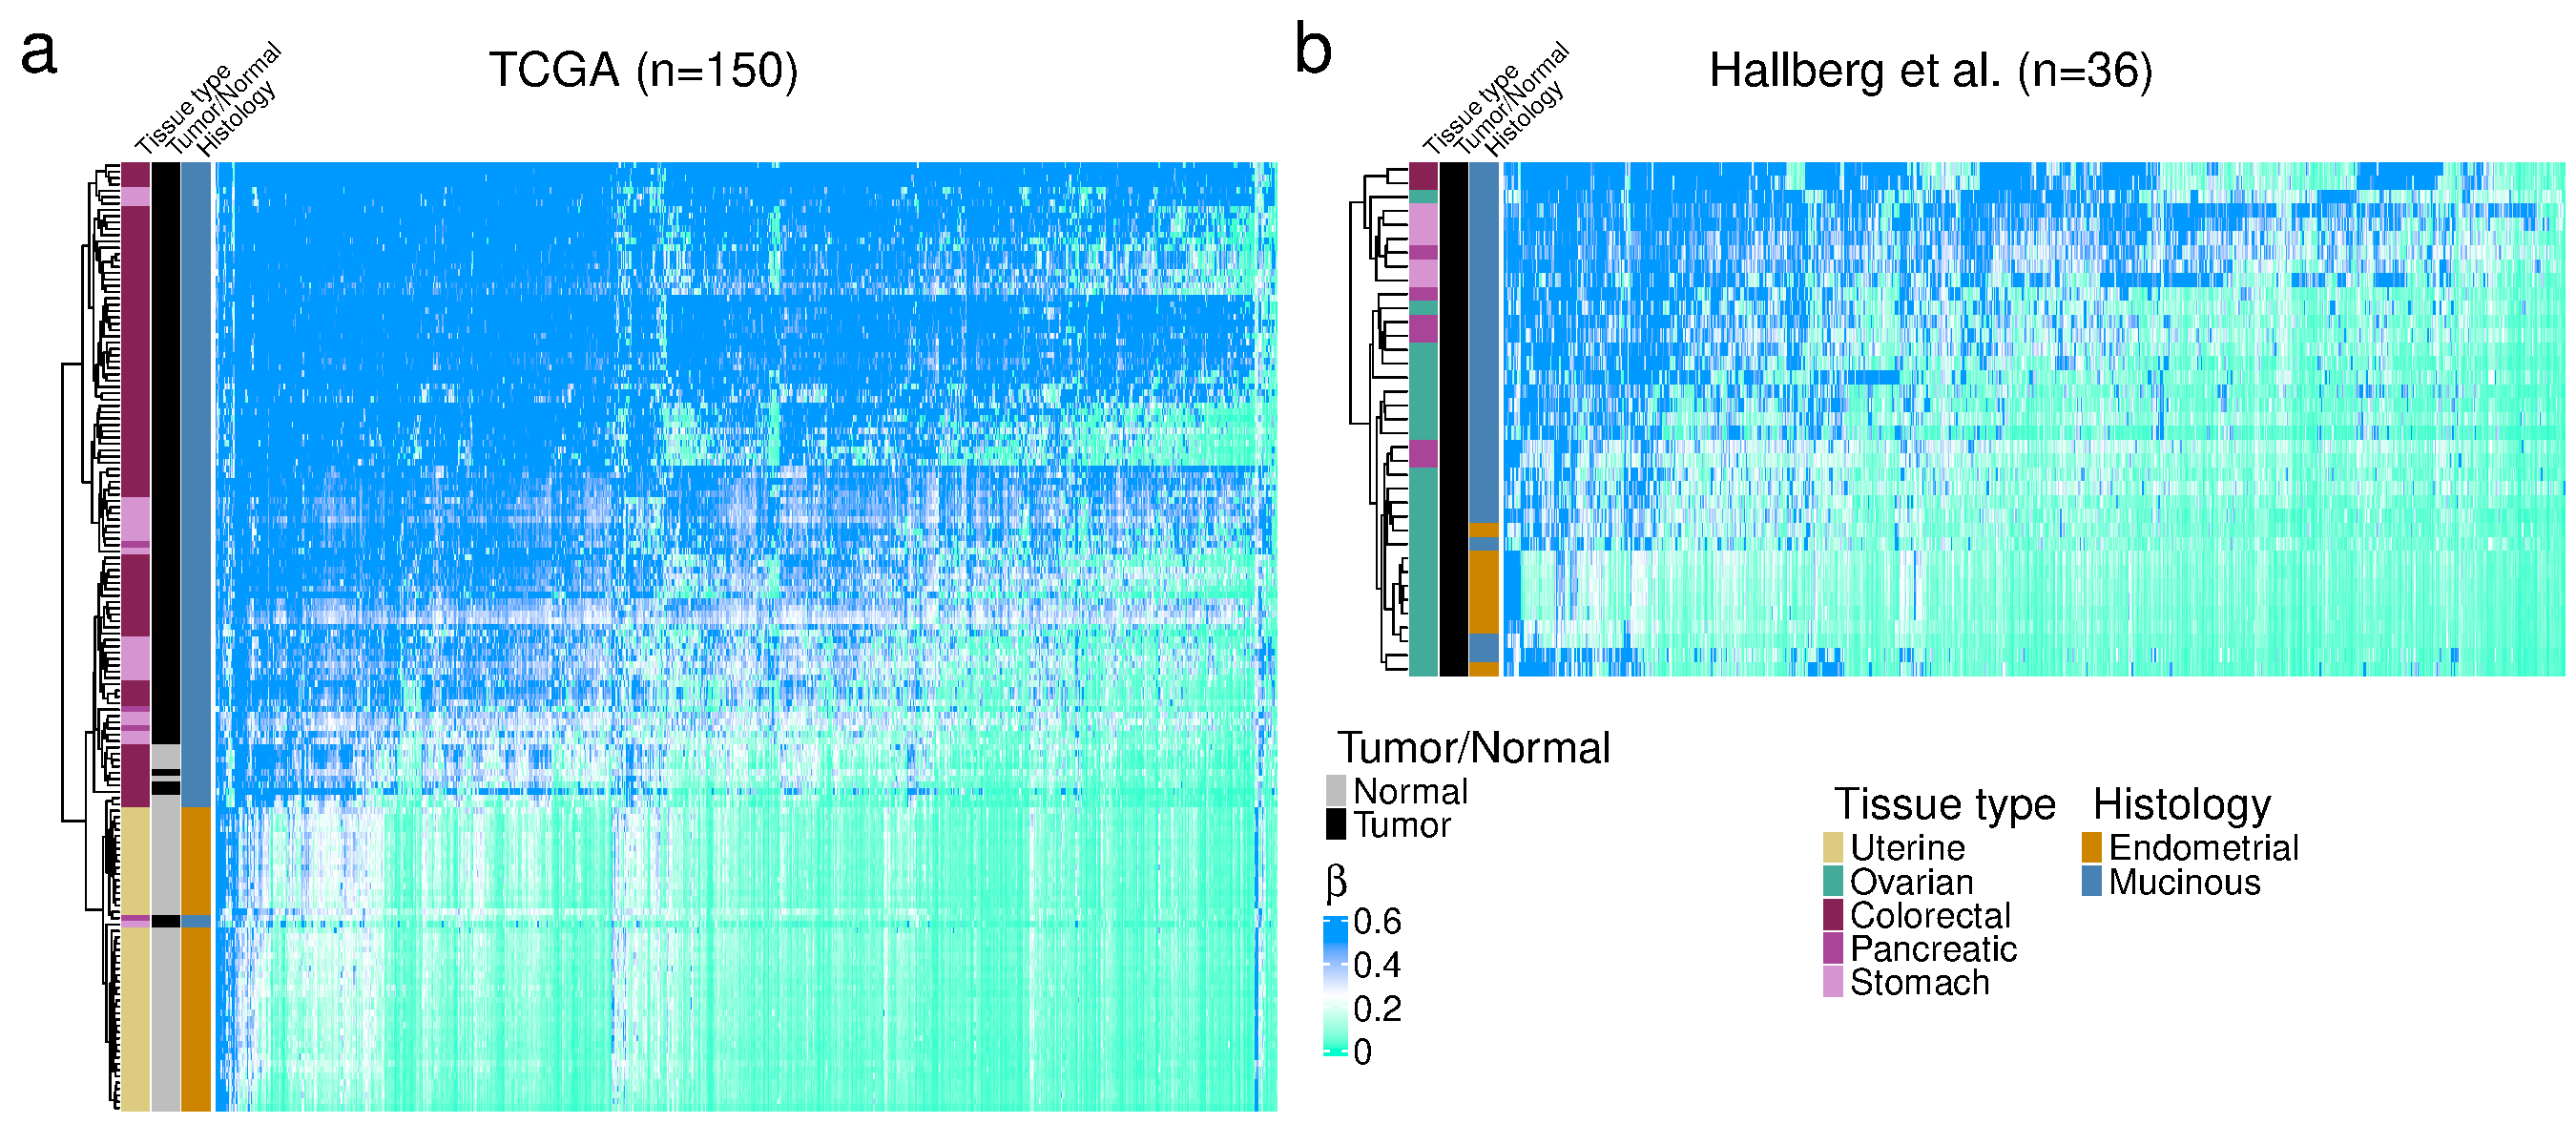
\includegraphics[width=\textwidth]{../docs/figure/ext-figure10.Rmd/heatmaps-1.pdf}
  \caption{\textbf{Heatmap of methylation values in mucinous and endometrial histotypes.}
    \textbf{(a)} Methylation levels ($\beta$s) at 945 CpG sites having the highest variance across 164 TCGA patient samples that included 77 colorectal mucinous tumors, 37 stomach mucinous tumors, and 46 uterine endometrial samples from normal tissue.   \textbf{(b)} Methylation levels at the same CpG sites were obtained from 16 patients with ovarian mucinous carcinomas, 8 patients with ovarian endometrioid carcinomas, 5 patients with stomach mucinous carcinomas, 6 patients with pancreatic mucinous carcinomas, and 1 patient with colorectal mucinous carcinoma.
    }
  \label{fig:sfig10}
\end{figure}

\begin{figure}
  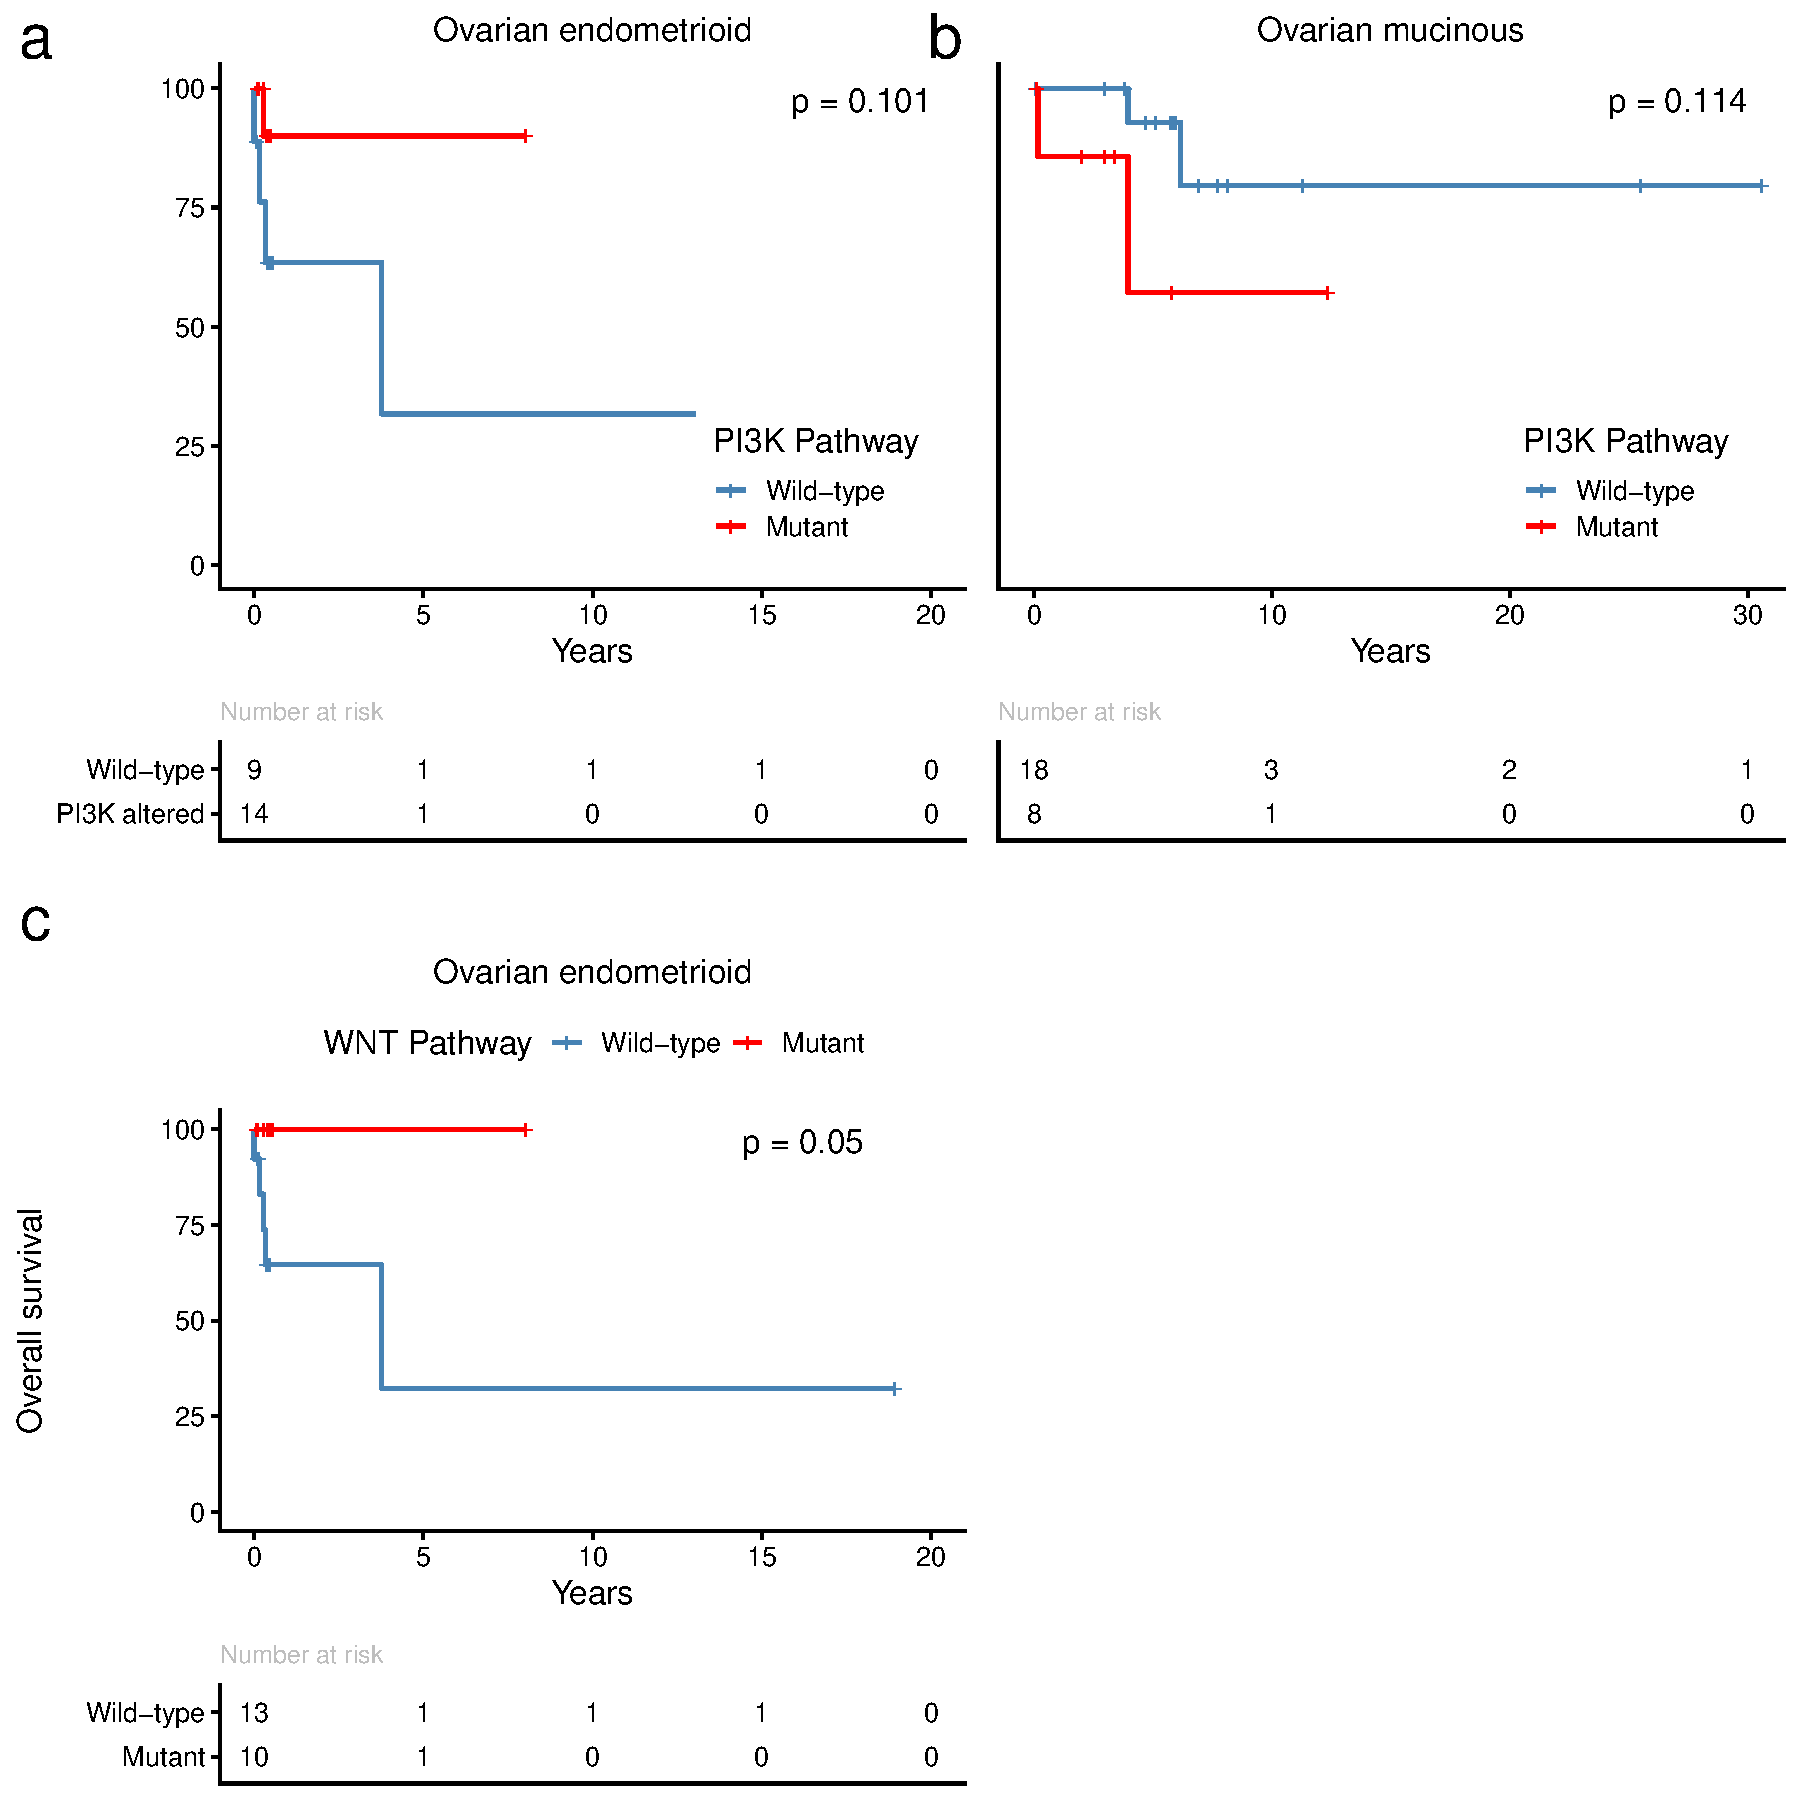
\includegraphics[height=6in]{../docs/figure/ext-figure11.Rmd/figS11-1.pdf}
  \caption{\textbf{Kaplan-Meier survival curves for ovarian cancer patients with and without mutations in the PI3K and WNT pathways.}
    \textbf{(a, b)} Alterations in the PI3K pathway trended towards increased survival among patients with ovarian endometrioid carcinomas and decreased survival among patients with ovarian mucinous carcinomas. \textbf{(c)} \textit{CTNNB1} alternations in the WNT pathway trended towards association with increased survival among patients with ovarian endometrioid carcinomas.}
  \label{fig:sfig11}
\end{figure}


\end{document}
